\documentclass[10pt,a4paper]{article}
\usepackage[utf8]{inputenc}
\usepackage[T1]{fontenc}
\usepackage[polish]{babel}
\let\babellll\lll
\let\lll\relax
\usepackage{polski}
\usepackage{graphicx}
\usepackage{todonotes}
\usepackage{listings}
\lstset{language=Matlab}
\usepackage{caption}
\usepackage[backend=biber]{biblatex}
\usepackage{multirow}

\usepackage[unicode,breaklinks,pdfusetitle,colorlinks=true]{hyperref}
\hypersetup{pdfproducer={Latex with hyperref},pdfcreator={pdflatex},allcolors=[rgb]{0,0,0.4}}
\addto\captionspolish{\renewcommand{\figurename}{Ilustracja}}

\author{Rafał Kabaciński}
\title{Technologie informacyjne\\Wprowadzenie do Matlaba}

\newcommand{\zadanie}[1]{\todo[inline,color=teal!20]{Zadanie: #1}}
\newcommand{\uwaga}[1]{\todo[inline,color=red!30]{Uwaga: #1}}

\lstset{
	literate=%
	{ą}{{\k{a}}}1
	{Ą}{{\k{A}}}1
	{ć}{{\'c}}1
	{Ć}{{\'{C}}}1
	{ę}{{\k{e}}}1
	{Ę}{{\k{E}}}1
	{ł}{{\l{}}}1
	{Ł}{{\L{}}}1
	{ń}{{\'n}}1
	{Ń}{{\'N}}1
	{ó}{{\'o}}1
	{Ó}{{\'O}}1
	{ś}{{\'s}}1
	{Ś}{{\'S}}1
	{ż}{{\.z}}1
	{Ż}{{\.Z}}1
	{ź}{{\'z}}1
	{Ź}{{\'Z}}1
}

\addbibresource{bibliografia.bib}

\begin{document}
	\maketitle
	\tableofcontents
	\section{Czym jest Matlab}
	
	Matlab to zintegrowane środowisko do obliczeń matematycznych, inżynierskich i prowadzenia symulacji oraz powiązanego z nim języka programowania. Jego nazwa wywodzi się od MATrix LABoratory, czyli laboratorium macierzy. Obecnie jednak jego możliwości wykraczają daleko poza obliczenia macierzowe, a sam program stosowany jest w wielu różnych dziedzinach. Poza podstawowym środowiskiem dostępne są liczne specjalizowane biblioteki narzędzi nazywane \emph{toolbox}ami. Pośród alternatyw dla Matlaba wyróżnia się otwarto-źródłowy pakiet Octave, którego jednym z celów jest kompatybilność z językiem Matlaba.
	
	Ponieważ pierwotnym przeznaczeniem środowiska było prowadzenie interaktywnych obliczeń, Matlab jest językiem interpretowanym a nie kompilowanym w przeciwieństwie do na przykład języków C, C++. 
		
	\section{Podstawy Matlaba}
	
	\subsection{Okno programu}
	
	Główne okno programu Matlab zaprezentowano na ilustracji~\ref{rys:M:Okno}.
	
	\begin{figure}[h!]
		\centering
		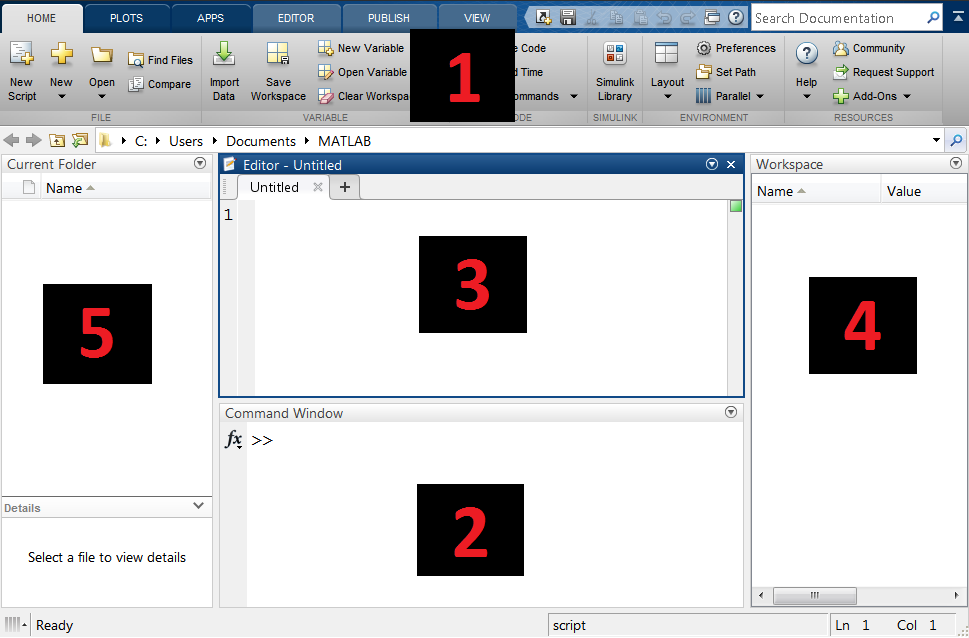
\includegraphics[width=1\textwidth]{Ilustracje/Matlab_Okno1.png}
		\caption[Okno programu Matlab]{Okno programu Matlab; 1~--~wstążki narzędzi, 2~--~linia komend, 3~--~edytor skryptów, 4~--~przestrzeń robocza, 5~--~pliki w bieżącym folderze}
		\label{rys:M:Okno}
	\end{figure}

	Narzędzia pogrupowane są w tak zwane wstążki, znajdujące się u góry okna (Ilustracja~\ref{rys:M:Okno}--1). Linia komend (Ilustracja~\ref{rys:M:Okno}--2) znajdująca się u dołu okna służy do prowadzenia interaktywnych obliczeń. Bardziej rozbudowane obliczenia umieścić można w plikach skryptów. Edytor takich plików znajduje się pośrodku (Ilustracja~\ref{rys:M:Okno}--3). Po prawej stronie znajduje się przestrzeń robocza ((Ilustracja~\ref{rys:M:Okno}--4), a po lewej podgląd plików w bieżącym folderze (Ilustracja~\ref{rys:M:Okno}--5).
	
	Jeżeli wygląd okna został zmieniony względem domyślnego, można go przywrócić. Służy do tego narzędzie \emph{Layout} znajdujące się po środku wstążki \emph{Home} (Ilustracja~\ref{rys:M:Okno2}).
	
	\begin{figure}[h!]
		\centering
		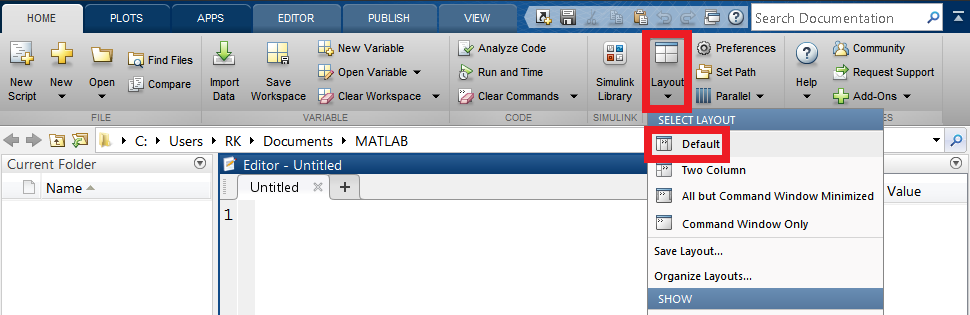
\includegraphics[width=1\textwidth]{Ilustracje/Matlab_Okno2.png}
		\caption{Przywrócenie domyślnej konfiguracji okna Matlaba}
		\label{rys:M:Okno2}
	\end{figure}

	Główne okno programu Octave ma zbliżoną konfigurację, zaprezentowane jest na ilustracji~\ref{rys:O:Okno}.
	
	\begin{figure}[h!]
		\centering
		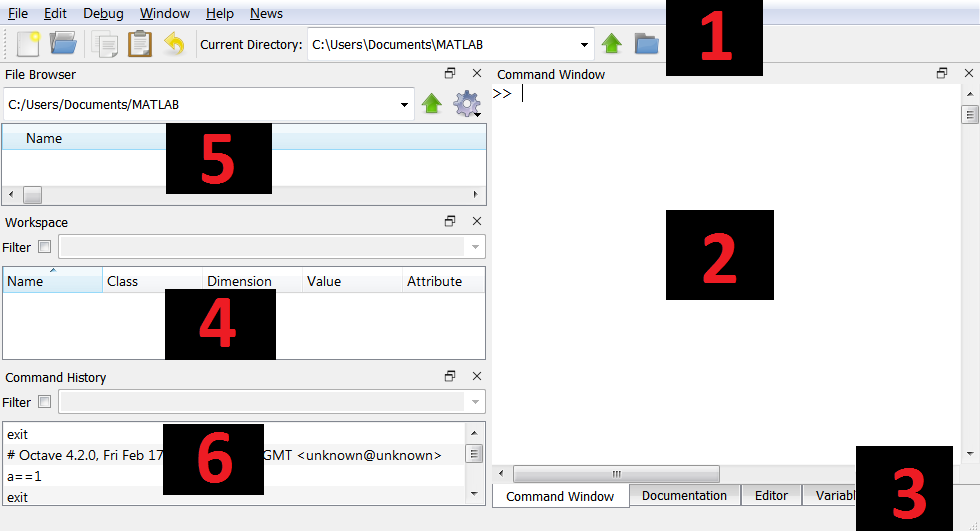
\includegraphics[width=1\textwidth]{Ilustracje/Octave_Okno1.png}
		\caption[Okno programu Octave]{Okno programu Octave; 1~--~narzędzia, 2~--~linia komend, 3~--~zakładki środkowego sub-okna, 4~--~przestrzeń robocza, 5~--~pliki w bieżącym folderze, 6~--~historia komend}
		\label{rys:O:Okno}
	\end{figure}


	Podstawowe narzędzia dostępne są u góry okna (Ilustracja~\ref{rys:O:Okno}--1). Linia komend (Ilustracja~\ref{rys:O:Okno}--2) znajduje się po prawej. Może ona być jednak przełączona między innymi na edytor skryptów za pomocą zakładek dostępnych u dołu okna (Ilustracja~\ref{rys:O:Okno}--3). Po lewej stronie, po środku znajduje się przestrzeń robocza ((Ilustracja~\ref{rys:M:Okno}--4). Nad nią z kolei umieszczono podgląd plików w bieżącym folderze (Ilustracja~\ref{rys:M:Okno}--5). Pod przestrzenią roboczą znajduje się sub-okno z historią komend.
	
	Jeżeli wygląd okna został zmieniony względem domyślnego, można go przywrócić. Służy do tego ostatnia opcja z menu \emph{Window} (Ilustracja~\ref{rys:O:Okno2}).
	
	\begin{figure}[h!]
		\centering
		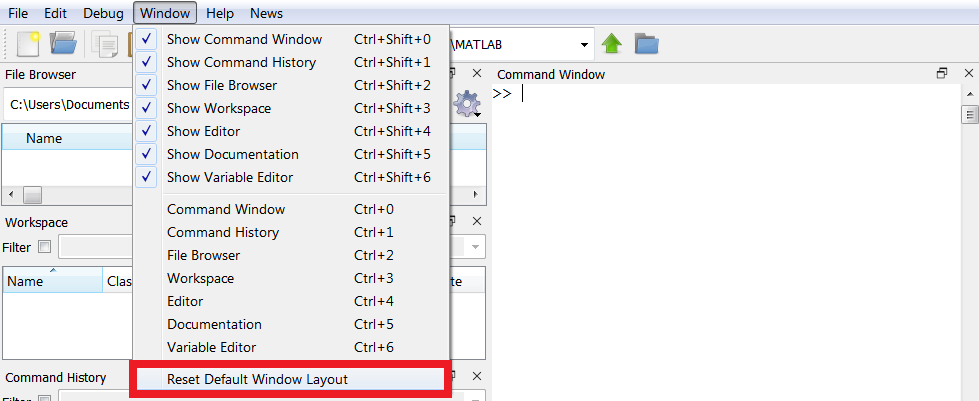
\includegraphics[width=1\textwidth]{Ilustracje/Octave_Okno2.png}
		\caption{Przywrócenie domyślnej konfiguracji okna Octave}
		\label{rys:O:Okno2}
	\end{figure}
	
	
		
	\section{Podstawowe komendy}
	
	\zadanie{wpisz:\\a==1\\w linii komend i wciśni enter.\\Przeczytaj informację o błędzie}
	
	Linia komend służy do prowadzenia interaktywnych obliczeń. Kolejne komendy potwierdza się za pomocą klawisza \emph{enter}. W przypadku błędu zamiast wyniku pojawia się informacja o błędzie zapisana czerwoną czcionką (czarną w Octave). Informacje te przeważnie szczegółowo informują jaki błąd pojawił się w komendzie, czasem sugerując nawet poprawki.
	
	\subsection{Praca ze zmiennymi}
	
	Do definiowania macierzy i wektorów służą nawiasy kwadratowe. Kolejne elementy w wierszu rozdziela się spacją bądź przecinkiem. Wiersze separuje się za pomocą średnika:
	\begin{lstlisting}
		a=[1 2]
		b=[1 2; 3 4]
	\end{lstlisting}
	
	\uwaga{Znak $=$ w większości języków programowania nie jest operatorem relacji równości jak w matematyce, tylko operatorem przypisania wartości po prawej do zmiennej po lewej jego stronie!}
	
	\zadanie{Zdefiniuj zmienne a i b jak w przykładzie}
	
	Zmienne zdefiniowane w trakcie sesji pojawiają się w przestrzeni roboczej. Można w niej sprawdzić nazwy, wymiary czy wartości (dla mniejszych macierzy). Typ zmiennym nadawany jest automatycznie przez środowisko zależnie od tego co zostanie do nich przypisane.
	
	Kolejne polecenia wpisane w linii komend zapisywane są do historii. Można się do nich odwołać za pomocą strzałek góra/dół na klawiaturze. W Matlabie wciśnięcie strzałki w górę wywołuje sub-okno historii, w Octave jest ono domyślnie widoczne cały czas po lewej stronie. Wywołane z historii komendy można edytować.
	
	Ciągi znakowe definiuje się za pomocą znaków apostrofu \emph{'} na początku i na końcu:
	
	\begin{lstlisting}
	str = 'ciag znakowy'
	\end{lstlisting}
	
	Średnik na końcu komendy oznacza wyłączenie echa, czyli pokazania wyniku w linii komend.
	
	\zadanie{Wpisz w linii komend:\\'test';\\Czy powyższy ciąg znakowy został gdziekolwiek zapisany?\\Podpowiedź: sprawdź w przestrzeni roboczej.}
	
	\subsection{Podstawowe działania}
	
	\zadanie{Spróbuj wymnożyć macierz b przez wektor a:\\a*b\\Przeczytaj informację o błędzie. Jak mnoży się macierze?}
	
	Podstawowe operatory w Matlabie wywołują działania macierzowe. O ile zawsze można wymnożyć skalar i macierz, o tyle macierze muszą mieć odpowiednie wymiary aby dane działanie dało się wykonać. Podstawowe operatory działań zaprezentowano w tabeli~\ref{tab:operatory_dzialan}.
	
	\begin{table}[h!]
		\centering
		\caption{Podstawowe operatory działań w Matlabie}
		\label{tab:operatory_dzialan}
		\begin{tabular}{c|c}
			Operator & Działanie \\ \hline
			+ & Dodawanie \\ \hline
			- & Odejmowanie \\ \hline
			* & Mnożenie \\ \hline
			/ & Dzielenie \\ \hline
			\verb|^| & Potęgowanie \\ \hline
			' & Transpozycja \\
		\end{tabular}
	\end{table}

	\zadanie{Wykorzystaj odpowiednie operatory aby wyliczyć iloczyny: skalarny i wektorowy zmiennej \emph{a} przez samą siebie.}

	Często zamiast działania macierzowego konieczne jest przeprowadzenie takiej samej operacji dla każdego elementu z osobna. W Matlabie w tym celu należy wstawić kropkę przed operatorem:
	\begin{lstlisting}
	b^2
	b.^2
	\end{lstlisting}
	
	\subsection{Definiowanie macierzy}
	
	Oprócz możliwości zdefiniowania całej macierzy ręcznie, pewne typy macierzy można zdefiniować za pomocą dedykowanych funkcji. Jak argumenty podaje się w nich kolejno liczbę wierszy i kolumn. Podanie jednej liczby jako argumentu będzie skutkować powstaniem macierzy kwadratowej. Funkcje te zaprezentowano w tabeli~ \ref{tab:def_macierzy}.
	
	\begin{table}[h!]
		\centering
		\caption{Funkcje definiujące macierze w Matlabie}
		\label{tab:def_macierzy}
		\begin{tabular}{c|c}
			Nazwa & Opis \\ \hline
			zeros(w,k) & Maciez zer \\ \hline
			ones(w,k) & Maciez jedynek \\ \hline
			eye(r) & Macierz jednostkowa \\ \hline
			rand(w,k) & Macierz losowych wartości z przedziału $\left\langle 0,1\right\rangle$ \\
		\end{tabular}
	\end{table}

	\zadanie{Korzystając z powyższych funkcji stwórz macierz zawierającą same liczby 5 o rozmiarach 4 na 6 (wiersze, kolumny)}
	
	\subsection{Podstawowe funkcje}
	
	Tabela~\ref{tab:podstawowe_funkcje} zawiera zestawienie podstawowych funkcji matematycznych w Matlabie.
	
	\begin{table}[h!]
		\centering
		\caption{Podstawowe funkcje matematyczne w Matlabie}
		\label{tab:podstawowe_funkcje}
		\begin{tabular}{c|c}
			Nazwa & Opis \\ \hline
			sin(a) & \multirow{4}{*}{funkcje trygonometryczne, argument w radianach} \\ 
			cos(a) &   \\ 
			tan(a) &   \\
			cot(a) & \\ \hline
			sind(a) & \multirow{4}{*}{funkcje trygonometryczne, argument w stopniach} \\ 
			cosd(a) &   \\ 
			tand(a) &   \\
			cotd(a) & \\ \hline
			sqrt(a) & pierwiastek kwadratowy \\ \hline
			exp(a) & funkcja eksponencjalna ($e^a$) \\ \hline
			log(a) & logarytm naturalny \\ \hline
			log10(a) & logarytm o podstawie 10 \\ \hline
			abs(a) & wartość bezwzględna \\ \hline
			pi & zwraca wartość liczby pi, nie przyjmuje argumentów \\ 
		\end{tabular}
	\end{table}

	\section{Skrypty}
	
	Dłuższe i bardziej skomplikowane obliczenia zapisywane są w skryptach. Są to pliki z rozszerzeniem \emph{*.m} zawierające komendy identyczne z tymi wprowadzanymi w linii komend. Skrypty uruchomić można w dwojaki sposób: za pomocą przycisku uruchom (ikona zielonego trójkąta, skrót klawiaturowy F5), na wstążce \emph{Editor} lub poprzez wpisanie nazwy skryptu w linii komend lub innym skrypcie. Nazwy zmiennych i skryptów obowiązują takie same zasady jak dla identyfikatorów w językach C, C++.
	
	\zadanie{Utwórz skrypt w nowym pod-folderze domyślnego folderu Matlaba. W skrypcie zapisz:\\
	c = a*b\\
	Następnie uruchom skrypt. Jakie pytanie zadaje Matlab/Octave?}
	\uwaga{W laboratorium zawsze należy wybrać opcję zmiany folderu, nigdy nie należy dodawać folderów do ścieżki!}
	
	Matlab uruchamia skrypty i funkcje z plików zapisanych na dysku nie z edytora. Narzędzie \emph{uruchom} zawsze najpierw zapisuje plik na dysku, dopiero potem uruchamia skrypt. Jeżeli wpisana zostanie nazwa nie będąca słowem kluczowym języka i nie będzie obecna w przestrzeni roboczej Matlab rozpoczyna szukanie pliku o takiej nazwie i rozszerzeniu \emph{.m} w folderach zapisanych w zmiennej \emph{path} i w folderze bieżącym. Poszukiwanie kończy się na pierwszym pliku, którego nazwa będzie zgodna. Folder bieżący można zamienić na inny, foldery dodane do ścieżki będą przeszukiwane za każdym razem.
	
	\zadanie{Czy po zamianie folderu skrypt zadziałał? Czy zmienna c pojawiła się w przestrzeni roboczej?}
	
	Skrypty (zasady nadawania nazw, jak i gdzie Matlab szuka funkcji, folder roboczy, współdzielenie przestrzeni roboczej?)

	 Skrypty współdzielą przestrzeń roboczą z użytkownikiem. Wszystkie zmienne zdefiniowane w linii komend są dostępne dla skryptów, a zmienne zdefiniowane w skryptach pojawiają się w przestrzeni użytkownika.
	 
	 \zadanie{Dopisz do skryptu linijkę:\\ z==0\\i uruchom skrypt}
	 
	 W przypadku wystąpienia błędu w skrypcie,informacja o nim zawiera hiperłącze do miejsca w edytorze w którym on wystąpił. Jest to fragment zapisany podkreśloną czcionką.
	 
	
	\section{Wykresy}
	
	\zadanie{Przepisz poniższy kod do własnego skryptu i uruchom.}
	\begin{lstlisting}
		x=[1 2 3 4];
		y=[1 2 3 4];
		plot(x,y,'-o')
		grid on
		axis tight
	\end{lstlisting}
		
	Do wyświetlania wykresów w Matlabie służy funkcja \emph{plot(x,y)}. Pierwszym argumentem jest wektor zawierający współrzędne odciętych (x), a drugim wektor zawierający współrzędne rzędnych (y). Kolejne punkty łączone są liniami prostymi
	
	\zadanie{Zmień wektor y na następujący:\\
	y=[1 2 1 2]\\
	Po obejrzeniu nowego wykresu zmień również wektor x na następujący:\\
	x=[1 2 2 1]}

	Funkcja plot nie sprawdza czy dany wykres jest funkcją więc możliwe jest rysowanie dowolnych krzywych.
	
	Trzecim argumentem funkcji plot jest ciąg formatujący. Może on zawierać specyfikację koloru i typu linii oraz typu markera w punktach danych.
	
	\zadanie{Wpisz w linii komend help plot i wciśnij enter}
	
	W temacie pomocy w linii komend, w pobliżu połowy wysokości można znaleźć wyszczególnienie jakie są możliwe opcje dla ciągu formatującego. Na dole tematu pomocy można znaleźć przykłady wykorzystania sprawdzanej komendy. Poniżej znajduje się hiperłącze do bardziej rozbudowanej pomocy otwieranej w osobnym oknie (Reference page for plot). Pomoc taką można otworzyć również wpisując doc plot, zamiast help plot.
	
	\zadanie{Otwórz temat pomocy w zewnętrznej przeglądarce i zapoznaj się z jej zawartością, zwłaszcza z listą tematów po lewej stronie i działem \emph{See Also} na dole.}
	
	Pomoc Matlaba jest dostępna również na stronach internetowych MathWorks, producenta Matlaba.
	
	Kolejne wywołania funkcji plot domyślnie nadpisują zawartość umieszczoną w poprzednim oknie rysunków. Można 
	zmienić to za pomocą polecenia:
	\begin{lstlisting}
	hold on
	\end{lstlisting}
	Jest ono przełącznikiem zmieniającym tryb działania okna. Po jego użyciu w danym oknie rysunkowym kolejne wywołania funkcji plot będą dodawać wykresy w tych samych osiach. Tryb ten można zmienić za pomocą polecenia:
	\begin{lstlisting}
	hold off
	\end{lstlisting}
	albo poprzez zamknięcie okna. Nowe okno rysunkowe otworzyć można za pomocą polecenia:
	\begin{lstlisting}
	figure
	\end{lstlisting}
	\uwaga{Polecenia plot, oraz pokrewne, rysują w ostatnim aktywnym oknie. Jeżeli użytkownik nie zamknie okna z poprzedniego uruchomienia skryptu wykres będzie dodany do poprzedniego okna i zostanie ono przesunięte na wierzch.}
	
	Pozostałe polecenia przydatne przy generowaniu wykresów:
	\begin{itemize}
		\item \lstinline|grid on| -- siatka pomocnicza,
		\item \lstinline|axis tight| -- usunięcie pustych przestrzeni wokół wykresu,
		\item \lstinline|axis equal| -- równe skale na osiach,
		\item \lstinline|title('Tytul')| -- tytuł wykresu,
		\item \lstinline|xlabel('x');ylabel('y')| -- etykiety osi,
		\item \lstinline|legend('zmienna1','zmienna2',...)| -- legenda,
		\item \lstinline|xlim([xmin xmax]);ylim([ymin ymax])| -- ustawienie zakresów na osiach.
	\end{itemize}
	
	
	\zadanie{Korzystając w wektora:\\t=1:0.01:1\\Przygotuj w skrypcie wykresy funkcji sinus o częstotliwościach $2$ i $3$ dla zakresu od $0$ do $2\pi$. Kolor linii ustaw na odpowiednio zielony i czerwony, dodaj tytuł wykresu, opisy osi, legendę w położeniu południowy-wschód, siatką pomocniczą i o zakresie osi y między $-1.2$ a $1.2$}
	
	
	%Close all, clear all, clc,
		 	
	%\section{Sterowanie przepływem}
	
	%	pętle w matlabie
	
%	\subsection{Wycinki}
	
	%\section{Funkcje}
	%Funkcje w Matlabie - różnice wzg. skryptów.
	
	%\section{Zapis do plików}
%	Zapis do plików (formatowanie danych tak żeby móc wstawić plik wynikowy bezpośrednio do LaTeXa jako tabelę).
	
%	\section{Simulink}

	
\end{document}